\documentclass[11pt]{article}
\newlength{\blackoutwidth}
\newcommand{\blackout}[1]
{%necessary comment
  \settowidth{\blackoutwidth}{#1}%necessary comment
  \rule[-0.3em]{\blackoutwidth}{1.125em}%necessary comment
}

\PassOptionsToPackage{usenames,dvipsnames}{xcolor}
\PassOptionsToPackage{colorlinks,linktoc=all}{hyperref}
\usepackage{balance}       % to better equalize the last page
\usepackage{graphics}      % for EPS, load graphicx instead 
\usepackage[T1]{fontenc}   % for umlauts and other diaeresis
\usepackage{txfonts}

\usepackage{color}
\usepackage{booktabs}
\usepackage{textcomp}
\usepackage{cuted}
\usepackage{capt-of}
\usepackage{bm}
\usepackage[pdflang={en-US},pdftex]{hyperref}

\title{Comparing Novel Machine Learning Methods For
Recommending Interesting Writing using a Controllable,
Explanation-Aware Visual Interface}
\author{Rohan Bansal}
\date{November 2020}

% !TEX root = ../regeneron.tex

% FONTS
%\usepackage[T1]{fontenc}

% Replace default Latin Modern typewriter with its proportional counterpart
% http://www.tug.dk/FontCatalogue/lmoderntypewriterprop/
%\renewcommand*\ttdefault{lmvtt}

%%% OPTION 3 - MTPRO 2 Math + Termes Times + ParaType Sans
\let\myBbbk\Bbbk
\let\Bbbk\relax
\let\bibsep\relax
\let\openbox\relax
\let\proof\relax
\let\endproof\relax
\let\iint\relax
\let\iiint\relax
\let\iiiint\relax
\let\idotsint\relax
%\usepackage{tgtermes}
\usepackage{minted}
\usepackage{amsmath}
\usepackage{blkarray}
% \usepackage[subscriptcorrection,
%             amssymbols,
%             mtpbb,
%             mtpcal,
%             nofontinfo  % suppresses all warnings
%            ]{mtpro2}
% \usepackage{scalefnt,letltxmacro}
% \LetLtxMacro{\oldtextsc}{\textsc}
% \renewcommand{\textsc}[1]{\oldtextsc{\scalefont{1.10}#1}}
% \usepackage[scaled=0.92]{PTSans}

% ICONS
\usepackage{fontawesome}

% CODE

% COLOR
\usepackage[usenames,dvipsnames]{xcolor}
\definecolor{shadecolor}{gray}{0.9}

% SPACING and TEXT
%\usepackage[final,expansion=alltext]{microtype}
%\usepackage[english]{babel}
\usepackage[parfill]{parskip}
\usepackage{afterpage}
\usepackage{framed}
\usepackage{nicefrac}

% EDITING
% line numbering in left margin
\usepackage{lineno}
\renewcommand\linenumberfont{\normalfont
                             \footnotesize
                             \sffamily
                             \color{SkyBlue}}
% ragged paragraphs in right margin
\usepackage{ragged2e}
\DeclareRobustCommand{\sidenote}[1]{\marginpar{
                                    \RaggedRight
                                    \textcolor{Plum}{\textsf{#1}}}}

% Define a paragraph header function
\DeclareRobustCommand{\parhead}[1]{\textbf{#1}~}

% paragraph helper
\DeclareRobustCommand{\PP}{\textcolor{Plum}{\P}~}
\DeclareRobustCommand{\pp}{\textcolor{Plum}{\P}~}

% COUNTERS
\renewcommand{\labelenumi}{\color{black!67}{\arabic{enumi}.}}
\renewcommand{\labelenumii}{{\color{black!67}(\alph{enumii})}}
\renewcommand{\labelitemi}{{\color{black!67}\textbullet}}

% FIGURES
\usepackage{graphicx}
\usepackage[labelfont=bf]{caption}
\usepackage[format=hang]{subcaption}

% TABLES
\usepackage{booktabs}
%\usepackage{dblfloatfix}  % for placing table at bottom of page

% TABLE ALIGNMENT
\usepackage{etoolbox,siunitx}
\robustify\bfseries
\sisetup{detect-weight=true, detect-shape=true, detect-mode=true,
table-format=5.1,
table-number-alignment=center,
separate-uncertainty=true,
input-ignore={,},input-decimal-markers={.}}

% BABEL
% \usepackage{polyglossia}


% ALGORITHMS
\usepackage[algoruled]{algorithm2e}
\usepackage{listings}
\usepackage{fancyvrb}
\fvset{fontsize=\normalsize}

% THEOREMS
\usepackage{amsthm}
\newtheorem{theorem}{Theorem}
% \newtheorem{proposition}[proposition]{Proposition}
\newtheorem{prop}{Proposition}


% TODO
%\usepackage{todo}

% HYPERREF
%\usepackage[colorlinks,linktoc=all]{hyperref}
\usepackage[all]{hypcap}
\hypersetup{citecolor=Violet}
\hypersetup{linkcolor=black}
\hypersetup{urlcolor=MidnightBlue}

% CLEVEREF must come after HYPERREF
\usepackage[capitalize]{cleveref}

% ACRONYMS
\usepackage[acronym,smallcaps,nowarn]{glossaries}
% \makeglossaries

% COLOR DEFINITIONS
\newcommand{\red}[1]{\textcolor{BrickRed}{#1}}
\newcommand{\orange}[1]{\textcolor{BurntOrange}{#1}}
\newcommand{\green}[1]{\textcolor{OliveGreen}{#1}}
\newcommand{\blue}[1]{\textcolor{MidnightBlue}{#1}}
\newcommand{\gray}[1]{\textcolor{black!60}{#1}}

% LISTINGS DEFINTIONS
\usepackage{listings}
\lstdefinestyle{alp_style}{
    commentstyle=\color{OliveGreen},
    numberstyle=\tiny\color{black!60},
    stringstyle=\color{BrickRed},
    basicstyle=\ttfamily\scriptsize,
    breakatwhitespace=false,
    breaklines=true,
    captionpos=b,
    keepspaces=true,
    numbers=none,
    numbersep=5pt,
    showspaces=false,
    showstringspaces=false,
    showtabs=false,
    tabsize=2
}
\lstset{style=alp_style}

\usepackage[margin=.8in,
includehead,
includefoot,]{geometry}

\usepackage{fancyhdr}
\pagestyle{fancy}
\fancyhf{}
\fancyfoot[R]{\thepage}
\renewcommand{\headrulewidth}{0pt}
\renewcommand{\footrulewidth}{0pt}

\usepackage[nottoc,numbib]{tocbibind}


% !TEX root = ../set_recommendation.tex

\DeclareRobustCommand{\mb}[1]{\ensuremath{\boldsymbol{\mathbf{#1}}}}
%\DeclareRobustCommand{\mb}[1]{\mathbold{#1}}

\DeclareRobustCommand{\KL}[2]{\ensuremath{\textrm{KL}\left(#1\;\|\;#2\right)}}

\DeclareMathOperator*{\argmax}{arg\,max}
\DeclareMathOperator*{\argmin}{arg\,min}

\newcommand{\yqm}{y_{qm}}
\newcommand{\xum}{x_{um}}
\newcommand{\xuk}{x_{uk}}
\newcommand{\yuk}{y_{uk}}
\renewcommand{\mid}{~\vert~}
\newcommand{\prm}{\:;\:}

\newcommand{\mbw}{\mb{w}}
\newcommand{\mbW}{\mb{W}}

\newcommand{\mbx}{\mb{x}}
\newcommand{\mbX}{\mb{X}}

\newcommand{\mby}{\mb{y}}
\newcommand{\mbY}{\mb{Y}}

\newcommand{\mbz}{\mb{z}}
\newcommand{\mbZ}{\mb{Z}}

\newcommand{\mbI}{\mb{I}}
\newcommand{\mbone}{\mb{1}}

\newcommand{\mbL}{\mb{L}}

\newcommand{\mbtheta}{\mb{\theta}}
\newcommand{\mbTheta}{\mb{\Theta}}
\newcommand{\mbomega}{\mb{\omega}}
\newcommand{\mbOmega}{\mb{\Omega}}
\newcommand{\mbsigma}{\mb{\sigma}}
\newcommand{\mbSigma}{\mb{\Sigma}}
\newcommand{\mbphi}{\mb{\phi}}
\newcommand{\mbPhi}{\mb{\Phi}}

\newcommand{\mbalpha}{\mb{\alpha}}
\newcommand{\mbbeta}{\mb{\beta}}
\newcommand{\mbgamma}{\mb{\gamma}}
\newcommand{\mbeta}{\mb{\eta}}
\newcommand{\mbmu}{\mb{\mu}}
\newcommand{\mbrho}{\mb{\rho}}
\newcommand{\mblambda}{\mb{\lambda}}
\newcommand{\mbzeta}{\mb{\zeta}}

\newcommand\dif{\mathop{}\!\mathrm{d}}
\newcommand{\diag}{\textrm{diag}}
\newcommand{\supp}{\textrm{supp}}

\newcommand{\E}{\mathbb{E}}
\newcommand{\V}{\mathbb{V}}
\newcommand{\bbH}{\mathbb{H}}

\newcommand{\bbN}{\mathbb{N}}
\newcommand{\bbZ}{\mathbb{Z}}
\newcommand{\bbR}{\mathbb{R}}
\newcommand{\bbS}{\mathbb{S}}

\newcommand{\cL}{\mathcal{L}}
\newcommand{\cS}{\mathcal{S}}
\newcommand{\cD}{\mathcal{D}}

\newcommand{\cN}{\mathcal{N}}
\newcommand{\cT}{\mathcal{T}}

\newcommand{\mult}{\textrm{Mult}}
\newcommand{\dirichlet}{\textrm{Dirichlet}}
\newcommand{\Gam}{\textrm{Gamma}}
\newcommand{\Pois}{\textrm{Poisson}}
% !TEX root = recommending-interesting-writing.tex

\newacronym{ELBO}{elbo}{evidence lower bound}
\newacronym{GMM}{gmm}{Gaussian mixture model}
\newacronym{KL}{kl}{Kullback-Leibler}
\newacronym{LDA}{lda}{latent Dirichlet allocation}
\newacronym{SVI}{svi}{stochastic variational inference}
\newacronym{DEF}{def}{deep exponential family}
\newacronym{rfs}{rfs}{\textsc{rankfromsets}}
\newacronym{bert}{bert}{\textsc{bert}}
\newacronym{NLP}{NLP}{natural language processing}
\newacronym{ctpf}{ctpf}{collaborative topic Poisson factorization}
% !TEX root = ../regeneron.tex

% from victor veitch

\usepackage[%
minnames=1,maxnames=99,maxcitenames=2,
style=numeric, %alphabetic, numeric, authoryear
giveninits=true, % true, false
hyperref,
natbib,
backend=biber,
sorting=nyt
]{biblatex}%

% suppress 'in'
\renewbibmacro{in:}{}

% \newbibmacro*{journal}{%
%   \iffieldundef{journaltitle}
%     {}
%     {\printtext[journaltitle]{%
%       \printfield[noformat]{journaltitle}%
%       \setunit{\subtitlepunct}%
%       \printfield[noformat]{journalsubtitle}}}}

% make lower case
% \DeclareFieldFormat[article,inbook,incollection,inproceedings,patent,thesis,unpublished]{titlecase}{\MakeSentenceCase*{#1}}


\bibliography{bib}
\begin{document}

% !TEX root = ../regeneron.tex
\begin{titlepage}
    \begin{center}
        \vspace*{3cm}
        

        \Large
        \textbf{Mathematics HL Investigation}

        \vspace{0.5cm}

        How can moments of inertias be mathematically derived for mass distributions with varying degrees of complexity?
            
        \vfill
            
            
            
    \end{center}
\end{titlepage}
\newpage

\tableofcontents
\newpage

% !TEX root = ../math_ia.tex
\section{Introduction}
\label{sec:introduction}
I first became intrigued with the concept of moment of inertia when learning about rotating bodies such as flywheels and ferris wheels. I understood that these bodies were "moving" and stored kinetic energy, but they had no linear movement, leaving me somewhat confused about the general premise for calculating their stored energy. I soon realized that an understanding of rotational movement and a particle based approach could higlight the parallels between linear kinetic energy and rotational kinetic energy which led to the discovery of moments of inertias. The literal definition of moment of inertia is the opposition of a body to having its speed of rotation abbout an axis altered by the application of a torque (the rotational equivalent of traditional inertia). It plays a major role in rotational dynamics and has a host of applications when it comes to motors, wheels, and machinery. Its ability to serve as a measure of the resistance to angular motion for a body makes it equally important as traditional inertia, which dictates many physical aspects of our daily lives. Pure rolling motion, bridge building, and flywheels in engines are all predicated on the concept of moment of inertia, and thus the idea becomes exceedingly crucial in the study and implementations of engineering. Scientists and mathematicians are continuing to look for methods to calculate more intricate moments of inertias to improve current physical systems and create new practical technology~\parencite{Young_Freedman_Young_2020}.


This interesting concept lends itself to a a mathematical investigation for deriving moment of inertia formulas for progressively more complex mass distributions. Because of the reliance of moment of inertia on the geometric makeup of a body, I decided to investigate the various approaches that are used to calculate the values and derive some of the most commonly used formulas in modern physics and mathematics. My combined interest in crucial physical applications, such as rotation, as well as the beauty of integration provide a clear motivation for the study and emphasize the personal nature of the investigation.

% !TEX root = ../math_ia.tex
\section{Background}
\label{sec:background}

\subsection{Kinetic Energy and Physics Definitions}
Kinetic energy is a measure of the energy of a moving body. The formula for the calculation of kinetic energy of a body moving with translational velocity $v$ and a mass $M$, with the assumption that the body is rigid and the center of mass is moving at the same constant velocity is shown in \cref{eq:basic_kinetic_energy}~\parencite{Young_Freedman_Young_2020}.

\begin{equation}
KE = \frac{1}{2}Mv^2
\label{eq:basic_kinetic_energy}
\end{equation}

For a complex body defined by a set of particle-masses with unique energies, the principle of superposition can be applied to produce \cref{eq:comb_kinetic_energy} in which the kinetic energies of each particle $i$ are summed.

\begin{equation}
KE = \sum_i\frac{1}{2}M_iv_i^2
\label{eq:comb_kinetic_energy}
\end{equation}

Thus, the calculation of kinetic energy of a rigid body exhibiting translational motion is based solely on mass and velocity and its geometric configuration has no impact on the quantity. However, for rotational motion, this premise can no longer be accepted because each particle has a unique linear velocity depending on its distance from the axis of rotation. Consider a thin disk rotating about a vertical axis that passes perpendicularly through its center as shown in \cref{fig:rotating_disk}.

% !TEX root = ../math_ia.tex
\begin{figure}[H]
  \centering
  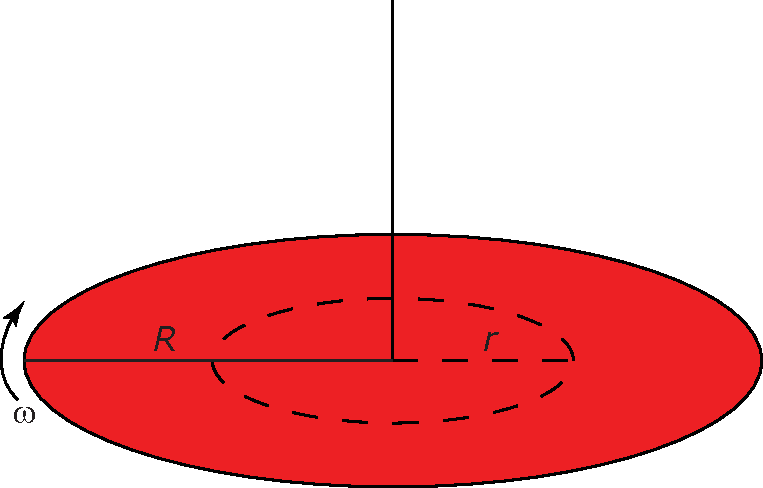
\includegraphics[width=0.35\linewidth]{fig/images/rotating_disk.pdf}
  \caption{A solid disk rotating about a centered, perpendicular axis with a constant angular velocity $\omega$}
  \label{fig:rotating_disk}
\end{figure}

Although each point of the disk is rotating with a constant angular velocity $\omega$, the linear velocity of each point is different. This can be easily determined using an understanding of rotation and time. The entire disk must undergo one complete revolution in time $\frac{2\pi}{\omega}$, but the distance that a point must travel in that time is dependent on its distance from the axis. For a point at a distance of $r$ from this axis, this distance is simply the circumfrence of a circle with radius $r$, or $2\pi r$. Using the formula $speed = \frac{distance}{time}$, the speed of this particle is defined by \cref{eq:v_and_w}. Thus, the rotating disk can actually be thought of as a combination of thin rings each consisting with particles moving at a unique velocity. 

\begin{equation}
v = \frac{2\pi r}{\frac{2\pi}{\omega}} = r\omega
\label{eq:v_and_w}
\end{equation}

For better generalization of this formula in instances where the velocity is not directly perpendicular to the axis of rotation, velocity can also be written as a cross product of the angular velocity vector (in the same direction as the axis of rotation) $\bm{\omega}$ and the position vector of the particle $\bm{r_i}$ as:

\begin{equation}
\bm{v_i} = \bm{\omega} \times \bm{r_i}
\end{equation}
and the angular velocity vector as:

\begin{equation}
\bm{\omega} = \omega \bm{k}
\end{equation}
where $\bm{k}$ is simply a unit vector in the direction of the rotational axis and $\omega$ is the magnitude of the angular velocity. Then, the velocity can simplified to:

\begin{equation}
\bm{v_i} = \omega |k \times \bm{r_i}|
\end{equation}

$|\bm{k} \times \bm{r_i}|$ is equivalent to the perpendicular distance between the point and the axis of rotation, which will be proved later. Using this value, we can utilize the traditional formula for kinetic energy to calculate the energy for a single rotating particle as:

\begin{equation}
R.K.E._i = \frac{1}{2}m_i\omega^2 |\bm{k} \times \bm{r_i}|^2
\label{eq:particle_rotational_energy}
\end{equation}

and the rotational energy for the entire body as:

\begin{equation}
R.K.E. = \sum_i \frac{1}{2}m_i\omega^2 |\bm{k} \times \bm{r_i}|^2
\label{eq:total_rotational_energy}
\end{equation}

To simplify this equation, the moment of inertia of a body is empirically defined as:

\begin{equation}
I = \sum_i m_i|\bm{k} \times \bm{r_i}|^2
\label{eq:total_moment_inertia}
\end{equation}

which for a single particle can be simplified to:

\begin{equation}
I = mr^2
\label{eq:simple_moment_inertia}
\end{equation}

where $r$ is the perpendicular distance from the particle to the axis.

The general formula for rotational kinetic energy can then be defined by \cref{eq:basic_rke} using two values, the rotational velocity $\omega$ and the moment of inertia $I$, which for a body rotating at a constant velocity about a fixed axis are constants (similar to $M$ and $v$ for traditional kinetic energy)~\parencite{Young_Freedman_Young_2020}.

\begin{equation}
R.K.E = \frac{1}{2}I\omega^2
\label{eq:basic_rke}
\end{equation}

Plugging in \cref{eq:simple_moment_inertia} and \cref{eq:v_and_w} to the equation for rotational kinetic energy shows that the final units remain the same as that for traditional kinetic energy presented in \cref{eq:basic_kinetic_energy}. Moment of inertias are also utilized to calculate angular momentum about a point which has many identical properties to traditional momentum, including conservation and collision governance. Using this information, I will derive moment of inertia formulas for a multitude of common bodies in motion.

\subsection{Vector Cross Products}

The formula for moment of inertia relies on the magnitude of a cross product. The general formula for the magnitude of a cross product is defined as~\parencite{Hass_Heil_Weir_2018}:

\begin{equation}
|\bm{u} \times \bm{v}| = |\bm{u}||\bm{v}|\sin{\theta}
\label{eq:cross_product}
\end{equation}

where $\theta$ is the angle between the two vectors.

This can be proved using basic vector rules:

\begin{gather*}
\text{Let } \bm{u} = \begin{bmatrix}u_1\\u_2\\u_3\end{bmatrix} \text{ and } \bm{v} = \begin{bmatrix}v_1\\v_2\\v_3\end{bmatrix} \\
\bm{u} \times \bm{v} = \begin{vmatrix}
\bm{i} & \bm{j} & \bm{j}\\
u_1 & u_2 & u_3 \\
v_1 & v_2 & v_3
\end{vmatrix} = \begin{vmatrix}
u_2 & u_3 \\
v_2 & v_3
\end{vmatrix}\bm{i} - \begin{vmatrix}
u_1 & u_3 \\
v_1 & v_3
\end{vmatrix}\bm{j} + \begin{vmatrix}
u_1 & u_2 \\
v_1 & v_2
\end{vmatrix}\bm{k} = \begin{bmatrix}u_2v_3 - u_3v_2\\u_3v_1 - u_1v_3\\u_1v_2 - u_2v_1\end{bmatrix}\\
\end{gather*}

Then, the squared-magnitude of the cross-product can be defined as:
\begin{align*}
|\bm{u} \times \bm{v}|^2 &= (\bm{u} \times \bm{v}) \cdot (\bm{u} \times \bm{v}) \\
&= (u_2v_3 - u_3v_2)^2 + (u_3v_1 - u_1v_3)^2 + (u_1v_2 - u_2v_1)^2 \\
&= u_2^2v_3^2 + u_3^2v_2^2 + u_1^2v_3^2 + u_3^2v_1^2 + u_1^2v_2^2 + u_2^2v_1^2 - 2(u_2u_3v_2v_3 + u_1u_3v_1v_3 + u_1u_2v_1v_2)
\end{align*}

We can also observe two other intriguing results:
\begin{align*}
(\bm{u} \cdot \bm{v})^2 &= (u_1v_1 + u_2v_2 + u_3v_3)^2 \\
&= u_1^2v_1^2 + u_2^2v_2^2 + u_3^2v_3^2 + 2(u_2u_3v_2v_3 + u_1u_3v_1v_3 + u_1u_2v_1v_2) \\
\end{align*}
\begin{align*}
(|\bm{u}||\bm{v}|)^2 &= (\sqrt{u_1^2 + u_2^2 + u_3^2}\sqrt{v_1^2 + v_2^2 + v_3^2})^2 \\
&= (u_1^2 + u_2^2 + u_3^2)(v_1^2 + v_2^2 + v_3^2) \\
&= u_2^2v_3^2 + u_3^2v_2^2 + u_1^2v_3^2 + u_3^2v_1^2 + u_1^2v_2^2 + u_2^2v_1^2 + u_1^2v_1^2 + u_2^2v_2^2 + u_3^2v_3^2
\end{align*}

By subtracting the second result from the third result, we can acquire the first result, leading to the formula:
\begin{align*}
|\bm{u} \times \bm{v}|^2 &= (|\bm{u}||\bm{v}|)^2 - (\bm{u} \cdot \bm{v})^2 \\
&= (|\bm{u}||\bm{v}|)^2 - (|\bm{u}||\bm{v}|\cos{\theta})^2 \\
&= (|\bm{u}||\bm{v}|)^2 - (|\bm{u}||\bm{v}|)^2\cos^2{\theta} \\
&= (|\bm{u}||\bm{v}|)^2(1 - \cos^2{\theta}) \\
&= (|\bm{u}||\bm{v}|)^2\sin^2{\theta}
\end{align*}

This result can then be square rooted, resulting in the initial theorem presented in \cref{eq:cross_product}. Because of this formula, the cross product between a unit vector and the position vector can also represent the perpendicular distance between the direction of the unit vector and the specific position. This premise is adopted for this investigation.

\subsection{Parallel Axis Theorem}

To calculate the moment of inertia for more complex bodies, the parallel axis theorem is often utilized to relate the moment of inertia about an axis passing through the center of mass of a body to a parallel axis at a distance $d$ from the central axis~\parencite{Abdulghany_2017}. \cref{eq:parallel_axis_formula} describes the theorem, where $I_{cm}$ is the moment of inertia through an axis passing through the center of mass, $M$ is the mass of the body, and $I'$ is the resultant moment of inertia through the parallel axis. This equation is applicable for any body, regardless of shape or dimensions.

\begin{equation}
I' = I_{cm} + Md^2
\label{eq:parallel_axis_formula}
\end{equation}

To prove this relationship, consider a lamina with mass $M$ located in the $X-Y$ plane whose center of mass is located at the origin as in \cref{fig:parallel_axis_lamina}. A general point $i$ is depicted and has coordinated $(x_i, y_i)$ and the parallel axis passes through $O$ which has coordinates $(a, b)$.

% !TEX root = ../math_ia.tex
\begin{figure}[H]
  \centering
  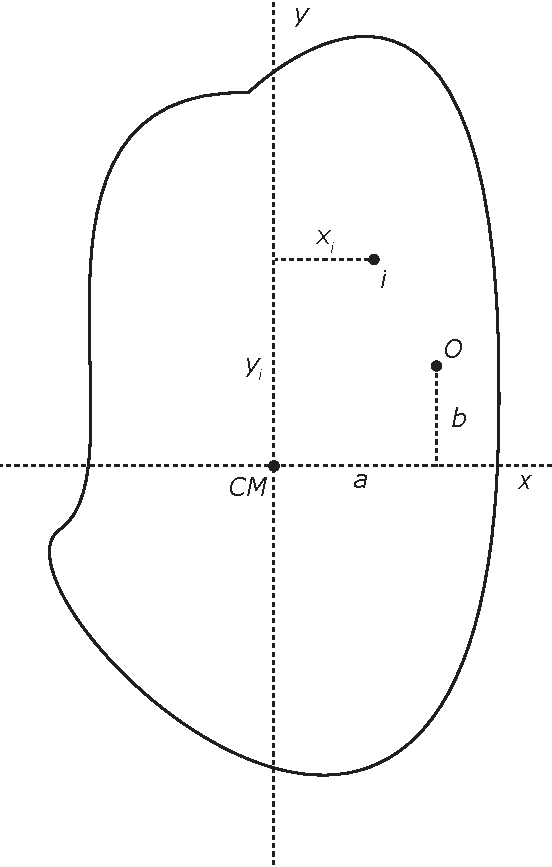
\includegraphics[width=0.25\linewidth]{fig/images/parallel_axis_lamina.pdf}
  \caption{A plain lamina in the $X-Y$ plane with its center of mass located at the origin}
  \label{fig:parallel_axis_lamina}
\end{figure} 

Because the center of mass is simply a weighted average of the mass of individual points on the lamina and the center of mass coincides with the origin, we can deduce:

\[x_{CM} = \frac{\sum_i m_ix_i}{M} = 0 \]
\[y_{CM} = \frac{\sum_i m_iy_i}{M} = 0 \]

Using the definition of moment of inertia for a particle and denoting the distance between point $i$ and point $O$ as $r_{iO}$, we can see $I_O = \sum_i m_i r_{iO}^2$. Using the distance formula, we have:

\[r_{iO}^2 = (x_i-a)^2 + (y_i-b)^2\]

Then,

\begin{align*}
I_O &= \sum_i m_i r_{iO}^2 \\
&= \sum_i m_i \left[(x_i-a)^2 + (y_i-b)^2\right] \\
&= \sum_i m_i \left[x_i^2 + a^2 - 2x_ia + y_i^2 + b^2 - 2y_ib\right]
\end{align*}

Now, using the deductions from the center of mass, the $2x_ia$ and $2y_ib$ terms can be removed, as $\frac{\sum_i m_ix_i}{M} = 0$ and $\frac{\sum_i m_iy_i}{M} = 0$, leaving:

\[I_O = \sum_i m_i (x_i^2 + y_i^2) + \sum_i m_i (a^2 + b^2) \]

Again, the distance formula (and the fact that the center of mass is located at the origin), allows us to see that $(x_i^2 + y_i^2)$ is simply equal to the square of the distance from point $i$ to the origin, or $r_i^2$, and $(a^2 + b^2)$ is equivalent to the square of the distance between point $O$ and the origin, or $d^2$. Then, we have:

\[I_O = \sum_i m_i r_i^2\ + \sum_i m_id^2\]

As we know that the first summation is equivalent to the moment of inertia about the center of mass (the origin) using \cref{eq:total_moment_inertia,eq:simple_moment_inertia}, and $d^2$ is constant, this simplifies to:

\[I_O = I_{CM} + Md^2\]

leaving the initial theorem as presented in \cref{eq:parallel_axis_formula}.


% !TEX root = ../math_ia.tex
\section{Derivations}
\label{sec:derivations}

\subsection{Hollow Ring/Cylinder}

Consider a hollow, uniform ring of radius $R$ and mass $M$ located in the $X-Y$ plane with its center at the origin rotating about the $Z$-axis as shown in \cref{fig:rotating_ring}.

% !TEX root = ../math_ia.tex
\begin{figure}[H]
  \centering
  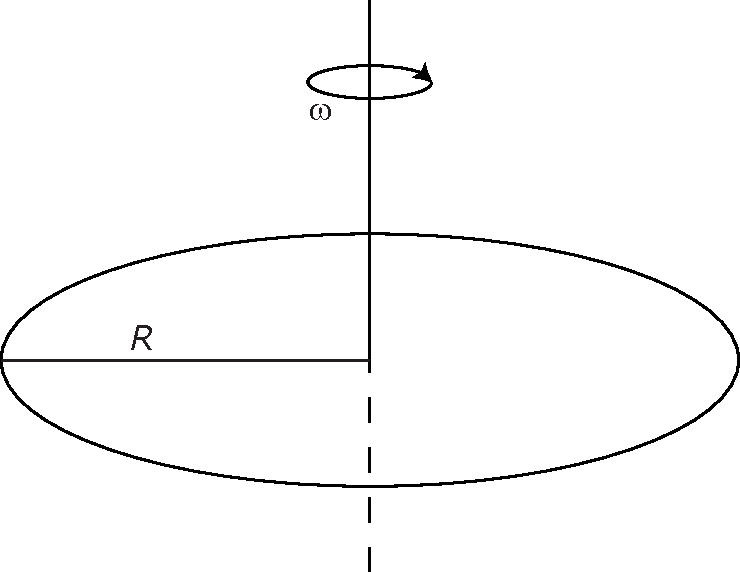
\includegraphics[width=0.25\linewidth]{fig/images/rotating_ring.pdf}
  \caption{A hollow ring rotating about a centered, perpendicular axis with a constant angular velocity $\omega$}
  \label{fig:rotating_ring}
\end{figure}

For this body, all particles are at a constant perpendicular distance from the axis of rotation, thus \cref{eq:total_moment_inertia} can be simplified to the following using the cross-product derivation:
\begin{gather*}
I = \sum_{i=1}^N m_i (|\bm{k}||\bm{r_i}| \sin{\frac{\pi}{2}})^2\\
\end{gather*}

As $\bm{k}$ is a unit vector, its magnitude is $1$ and the magnitude of $\bm{r_i}$ is simply $R$  \begin{gather*}  
I = \sum_{i=1}^N m_i (1 \times R \times 1)^2 \\
I = \sum_{i=1}^N m_i R^2
\end{gather*}

Since the $R^2$ term is constant for all mass particles, the term can be removed from the summation and the inner term is simply summing over the mass of the body:
\begin{align*}
I = R^2\sum_{i=1}^N m_i \\
I = R^2 \times M \\
\end{align*}

Thus, the moment of inertia for a hollow ring has been extrapolated leaving only the overall mass and radius in the formula, as shown in \cref{eq:final_moment_ring}.
\begin{equation}
I_{\text{ring}} = MR^2
\label{eq:final_moment_ring}
\end{equation}

A similar premise can be adopted for a hollow cylinder, with radius $R$ and mass $M$, centered at the origin and rotating around the $Z$-axis as shown in \cref{fig:rotating_hollow_cylinder}.

% !TEX root = ../math_ia.tex
\begin{figure}[H]
  \centering
  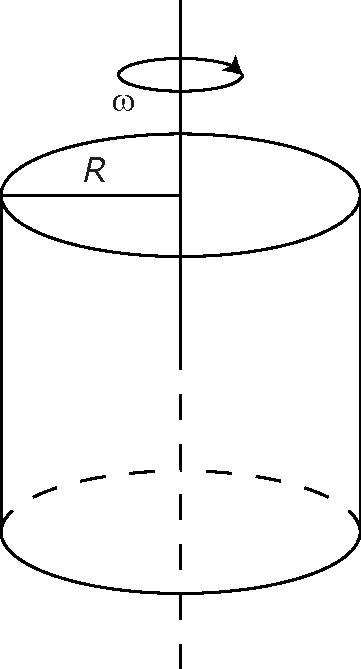
\includegraphics[width=0.25\linewidth]{fig/images/rotating_hollow_cylinder.pdf}
  \caption{A hollow cylinder rotating about a centered, perpendicular axis with a constant angular velocity $\omega$}
  \label{fig:rotating_hollow_cylinder}
\end{figure}

As the perpendicular distance between each point and the axis of rotation is once again a constant $R$, the final result for the moment of inertia will be identical:

\begin{equation}
I_{\text{hollow cylinder}} = MR^2
\label{eq:final_moment_hollow_cylinder}
\end{equation}

\subsection{Solid Cylinder}

For a solid, uniform cylinder of mass $M$, height $L$ and radius $R$, the process becomes more complicated due to the initial problem discussed in the background--different particles having different distances from the axis of rotation. Consider a cylinder as shown in \cref{fig:rotating_solid_cylinder}.

% !TEX root = ../math_ia.tex
\begin{figure}[H]
  \centering
  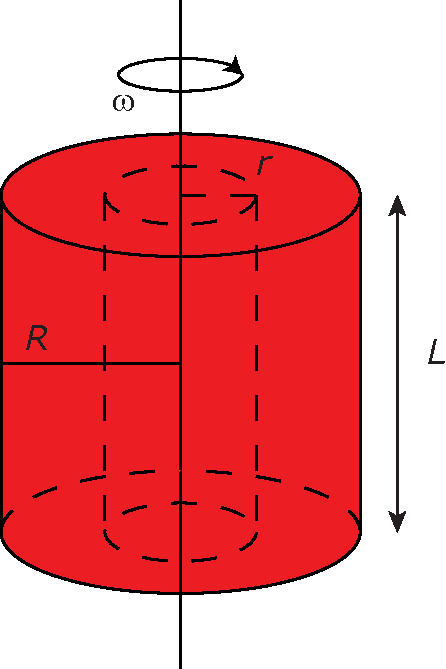
\includegraphics[width=0.25\linewidth]{fig/images/rotating_solid_cylinder.pdf}
  \caption{A solid cylinder rotating about a centered, perpendicular axis with a constant angular velocity $\omega$. A small shell of radius $r$ has also been depicted for visualization purposes}
  \label{fig:rotating_solid_cylinder}
\end{figure}

Assume the cylinder to have a constant density $\rho$, which leads to the determination:
\begin{gather*}
density = \frac{Mass}{Volume} = \frac{M}{V} \\
V = \pi R^2L \\
\rho = \frac{M}{\pi R^2L}\\
\end{gather*}
Consider the thin cylindrical shell formed from all the particles at a distance of $r$ from the axis of rotation, with a thickness $dr$ and a mass $dm$. Each of these shells' moment of inertia can then easily be transformed into an integral:
\begin{equation}
I = \int_0^M r^2dm
\end{equation}
as the perpendicular distance is represented by $r$ and the mass elements $dm$ are being summed over for the entire mass of the body. It is important to note, however, that $r$, $dm$ and $r^2$ are not constant in this integral, as they will depend on the specific shell. Thus, we must reduce from two variables down to one to solve for the moment of inertia.

The mass of shell can be represented as:
\begin{gather*}
dm = \rho dV \text{ (as mass} = \text{volume} \times \text{density)} \\
\end{gather*}
We can calculate $dV$ using the fact that the cylindrical shell has an infinitesimally small thickness. The shell can be cut and unfolded into a rectangular prism, with a width equal to the circumfrence of the shell, a thickness of $dr$, and a constant length of $L$:
\begin{gather*}
V = AL \\
dV = dAL \\
dV = 2\pi r dr L
\end{gather*}
Plugging this back into our formula for $dm$, we have:
\begin{gather*}
dm = \rho dV \\
dm = \rho 2\pi r dr L
\end{gather*}
As the distance of the shells from the axis of rotation ranges from $0$ to $R$, we must integrate over this interval while removing constants, resulting in:
\begin{gather*}
I = \int_0^R 2\pi\rho L r^3dr \\
I = 2\pi\rho L\int_0^R r^3dr \\
I = 2\pi\rho L\left[\frac{r^4}{4}\right]_0^R \\
I = 2\pi\rho\frac{R^4}{4}
\end{gather*}
Plugging in the initial value for $\rho$ calculated above, the resulting equation for the moment of inertia of a cylinder (using only the defined quantities of mass and total radius) is determined to be:
\begin{equation}
I_{\text{solid cylinder}} = \frac{1}{2}MR^2
\label{eq:final_moment_solid_cylinder}
\end{equation}

It is also important to note that this final formula for a cylinder is not dependent on the height $L$ of the cylinder, and thus the moment of inertia for a solid disk or cylindrical shape of any height can be calculated with this simple equation.

\subsection{Solid Sphere}

A similar approach can then be employed for other solid shapes that can be broken down into shells or disks, such as a solid sphere with mass $M$ and radius $R$ shown in \cref{fig:rotating_solid_sphere}.

% !TEX root = ../math_ia.tex
\begin{figure}[H]
  \centering
  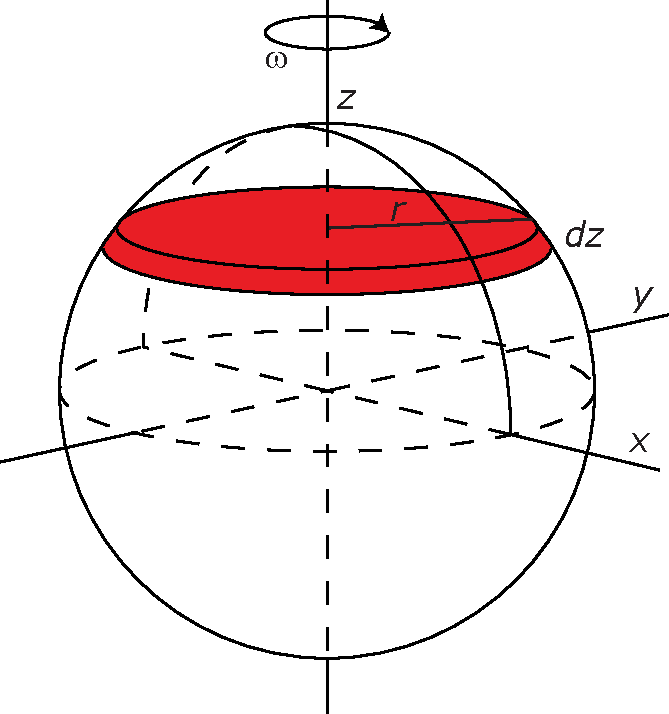
\includegraphics[width=0.25\linewidth]{fig/images/rotating_solid_sphere.pdf}
  \caption{A solid sphere centered at the origin rotating about the $Z$-axis with a constant angular velocity $\omega$. A small disk of radius $r$ has also been depicted for visualization purposes}
  \label{fig:rotating_solid_sphere}
\end{figure}

Again, assume the cylinder to have a constant density $\rho$, which can be written as:

\[\rho = \frac{M}{\frac{4}{3}\pi R^3}\]

Considering the thin disk with a radius $r$, we can write the infinitesmal moment of inertia for this disk by differentiating \cref{eq:final_moment_solid_cylinder}:

 \[dI = \frac{1}{2}r^2dm = \frac{1}{2}r^2\rho dV\]

 To calculate $dV$, a similar approach can be adopted by using the relation $V = A \times H$ and the fact that the height of this infinitesmal disk is simply $dz$:

 \[dV = \pi r^2 dz\]

 We can also relate the value of $z$, representing the height, with the value of $r$, representing the radius of the disk, using basic right-triangle geometry as the distance of all points on the sphere must be a distance of $R$ from the origin:

 \[r^2 + z^2 = R^2\]
 \[r^2 = R^2 - z^2\]

Plugging our values for $dV$ and $r^2$ back in and integrating from $-R$ to $R$ to travel from the bottom to the top of the sphere:

\[dI  = \frac{1}{2}r^2\rho dV = \frac{1}{2}r^2\rho \pi r^2 dz\]
\[I = \frac{1}{2}\rho \pi \int_{-R}^R r^4 dz\]
\[I = \frac{1}{2}\rho \pi \int_{-R}^R (R^2 - z^2)^2 dz\]
\[I =\frac{1}{2}\rho \pi \int_{-R}^R (R^4 + z^4 - 2R^2z^2) dz\]
\[I = \frac{1}{2}\rho \pi \left[\frac{z^5}{5} - \frac{2}{3}R^2z^3 + R^4z\right]_{-R}^{R}\]
\[I = \frac{8}{15}\rho \pi R^5\]

Substituting the initial value for $\rho$, the equation for the moment of inertia of solid cylinder can be derived as:

\begin{equation}
I_{\text{solid sphere}} = \frac{2}{5}MR^2
\label{eq:final_moment_solid_sphere}
\end{equation}

\cleardoublepage
\printbibliography

\end{document}{}
